\documentclass[aspectratio=169]{beamer}
% --------------------------------------------- %
% Pacote de estilo da UDESC
\usepackage{style/udesc}
\usepackage{listings}
\usepackage{hyperref}
\setbeamertemplate{itemize items}[circle]
\usepackage[abnt-emphasize=bf,abnt-and-type=e,alf]{abntex2cite}%Citações ABNT


% Incluir arquivos da pasta figuras
\graphicspath{{./img/}}

\setbeamertemplate{frametitle continuation}{}

% aPacote de texto aleatório
\usepackage{lipsum}

\lstset{ 
	basicstyle=\footnotesize,        % the size of the fonts that are used for the code
	breakatwhitespace=false,         % sets if automatic breaks should only happen at whitespace
	breaklines=true,                 % sets automatic line breaking
	captionpos=b,                    % sets the caption-position to bottom
	deletekeywords={...},            % if you want to delete keywords from the given language
	escapeinside={\%*}{*)},          % if you want to add LaTeX within your code
	extendedchars=true,              % lets you use non-ASCII characters; for 8-bits encodings only, does not work with UTF-8
	firstnumber=0,                % start line enumeration with line 1000
	frame=single,	                   % adds a frame around the code
	keepspaces=true,                 % keeps spaces in text, useful for keeping indentation of code (possibly needs columns=flexible)
	language=Java,                 % the language of the code
	morekeywords={*,...},            % if you want to add more keywords to the set
	numbers=none,                    % where to put the line-numbers; possible values are (none, left, right)
	numbersep=0pt,                   % how far the line-numbers are from the code
	rulecolor=\color{black},         % if not set, the frame-color may be changed on line-breaks within not-black text (e.g. comments (green here))
	showspaces=false,                % show spaces everywhere adding particular underscores; it overrides 'showstringspaces'
	showstringspaces=false,          % underline spaces within strings only
	showtabs=false,                  % show tabs within strings adding particular underscores
	stepnumber=2,                    % the step between two line-numbers. If it's 1, each line will be numbered
	tabsize=1,	                   % sets default tabsize to 2 
	basicstyle=\fontsize{7}{8}\selectfont\ttstyle,
	keywordstyle=\color{blue},
	commentstyle=\fontsize{7}{8}\selectfont\ttstyle\color{gray},
	stringstyle=\color{orange},
}

% Início do documento
\begin{document}
\usetikzlibrary{positioning}
\usetikzlibrary{shadows.blur, trees}
\definecolor{greenudesc}{HTML}{01934A}

%%
%%	Incluir \capa para os slides
%% 
\titulo{Distribuições Partônicas}
\subtitulo{Parametrizações}
\newcommand{\autor}{Rodrigo Ribamar Silva do Nascimento}
\newcommand{\github}{github.com/physikices}
\newcommand{\email}{rodrigo.nascimento@edu.udesc.br}
\newcommand{\website}{}
\frase{2023 - IC Física de Partículas}
\universidade{Universidade do Estado de Santa Catarina}
\capa

\AtBeginSection[]{
	\begin{frame}<beamer>
		\frametitle{Seções}
		\tableofcontents[currentsection]
\end{frame}}
\section{Introdução}
\section{A Estrutura dos Hádrons}
\subsection{DIS}
\subsection{DIS no modelo de Pártons}
\subsection{As Equações de Evolução -- DGLAP}
\section{Simulação Numérica}
\subsection{Produção de Méson Vetorial}
\subsection{Produção \texorpdfstring{$J/\psi$}{lg} com correções da LO}

% --------------------------------------------- %
% Introdução
% --------------------------------------------- %
\begin{frame}[plain]
	\tikzset{
		udesc greenBox/.style = {
			thin,
			blur shadow={
				shadow blur steps=10,
				shadow blur extra rounding=2pt, 
				shadow xshift=1pt
			},
			rectangle,
			minimum width=14em,
			minimum height=20mm,
			fill=greenudesc,
			text centered,
			anchor=base,
			inner sep=2ex
		},
	}
	\begin{tikzpicture}[remember picture,overlay]
		\node
			[udesc greenBox,yshift=-25pt,xshift=20pt] (box){}; 
		\node [right of = box, align=right,text=white] { {\LARGE Introdução}\\O Modelo Padrão};
	\end{tikzpicture}
\end{frame}
\begin{frame}{Introdução}
	\framesubtitle{O Modelo Padrão para a Física de Partículas}
	\begin{figure}[htb!]
		\centering
		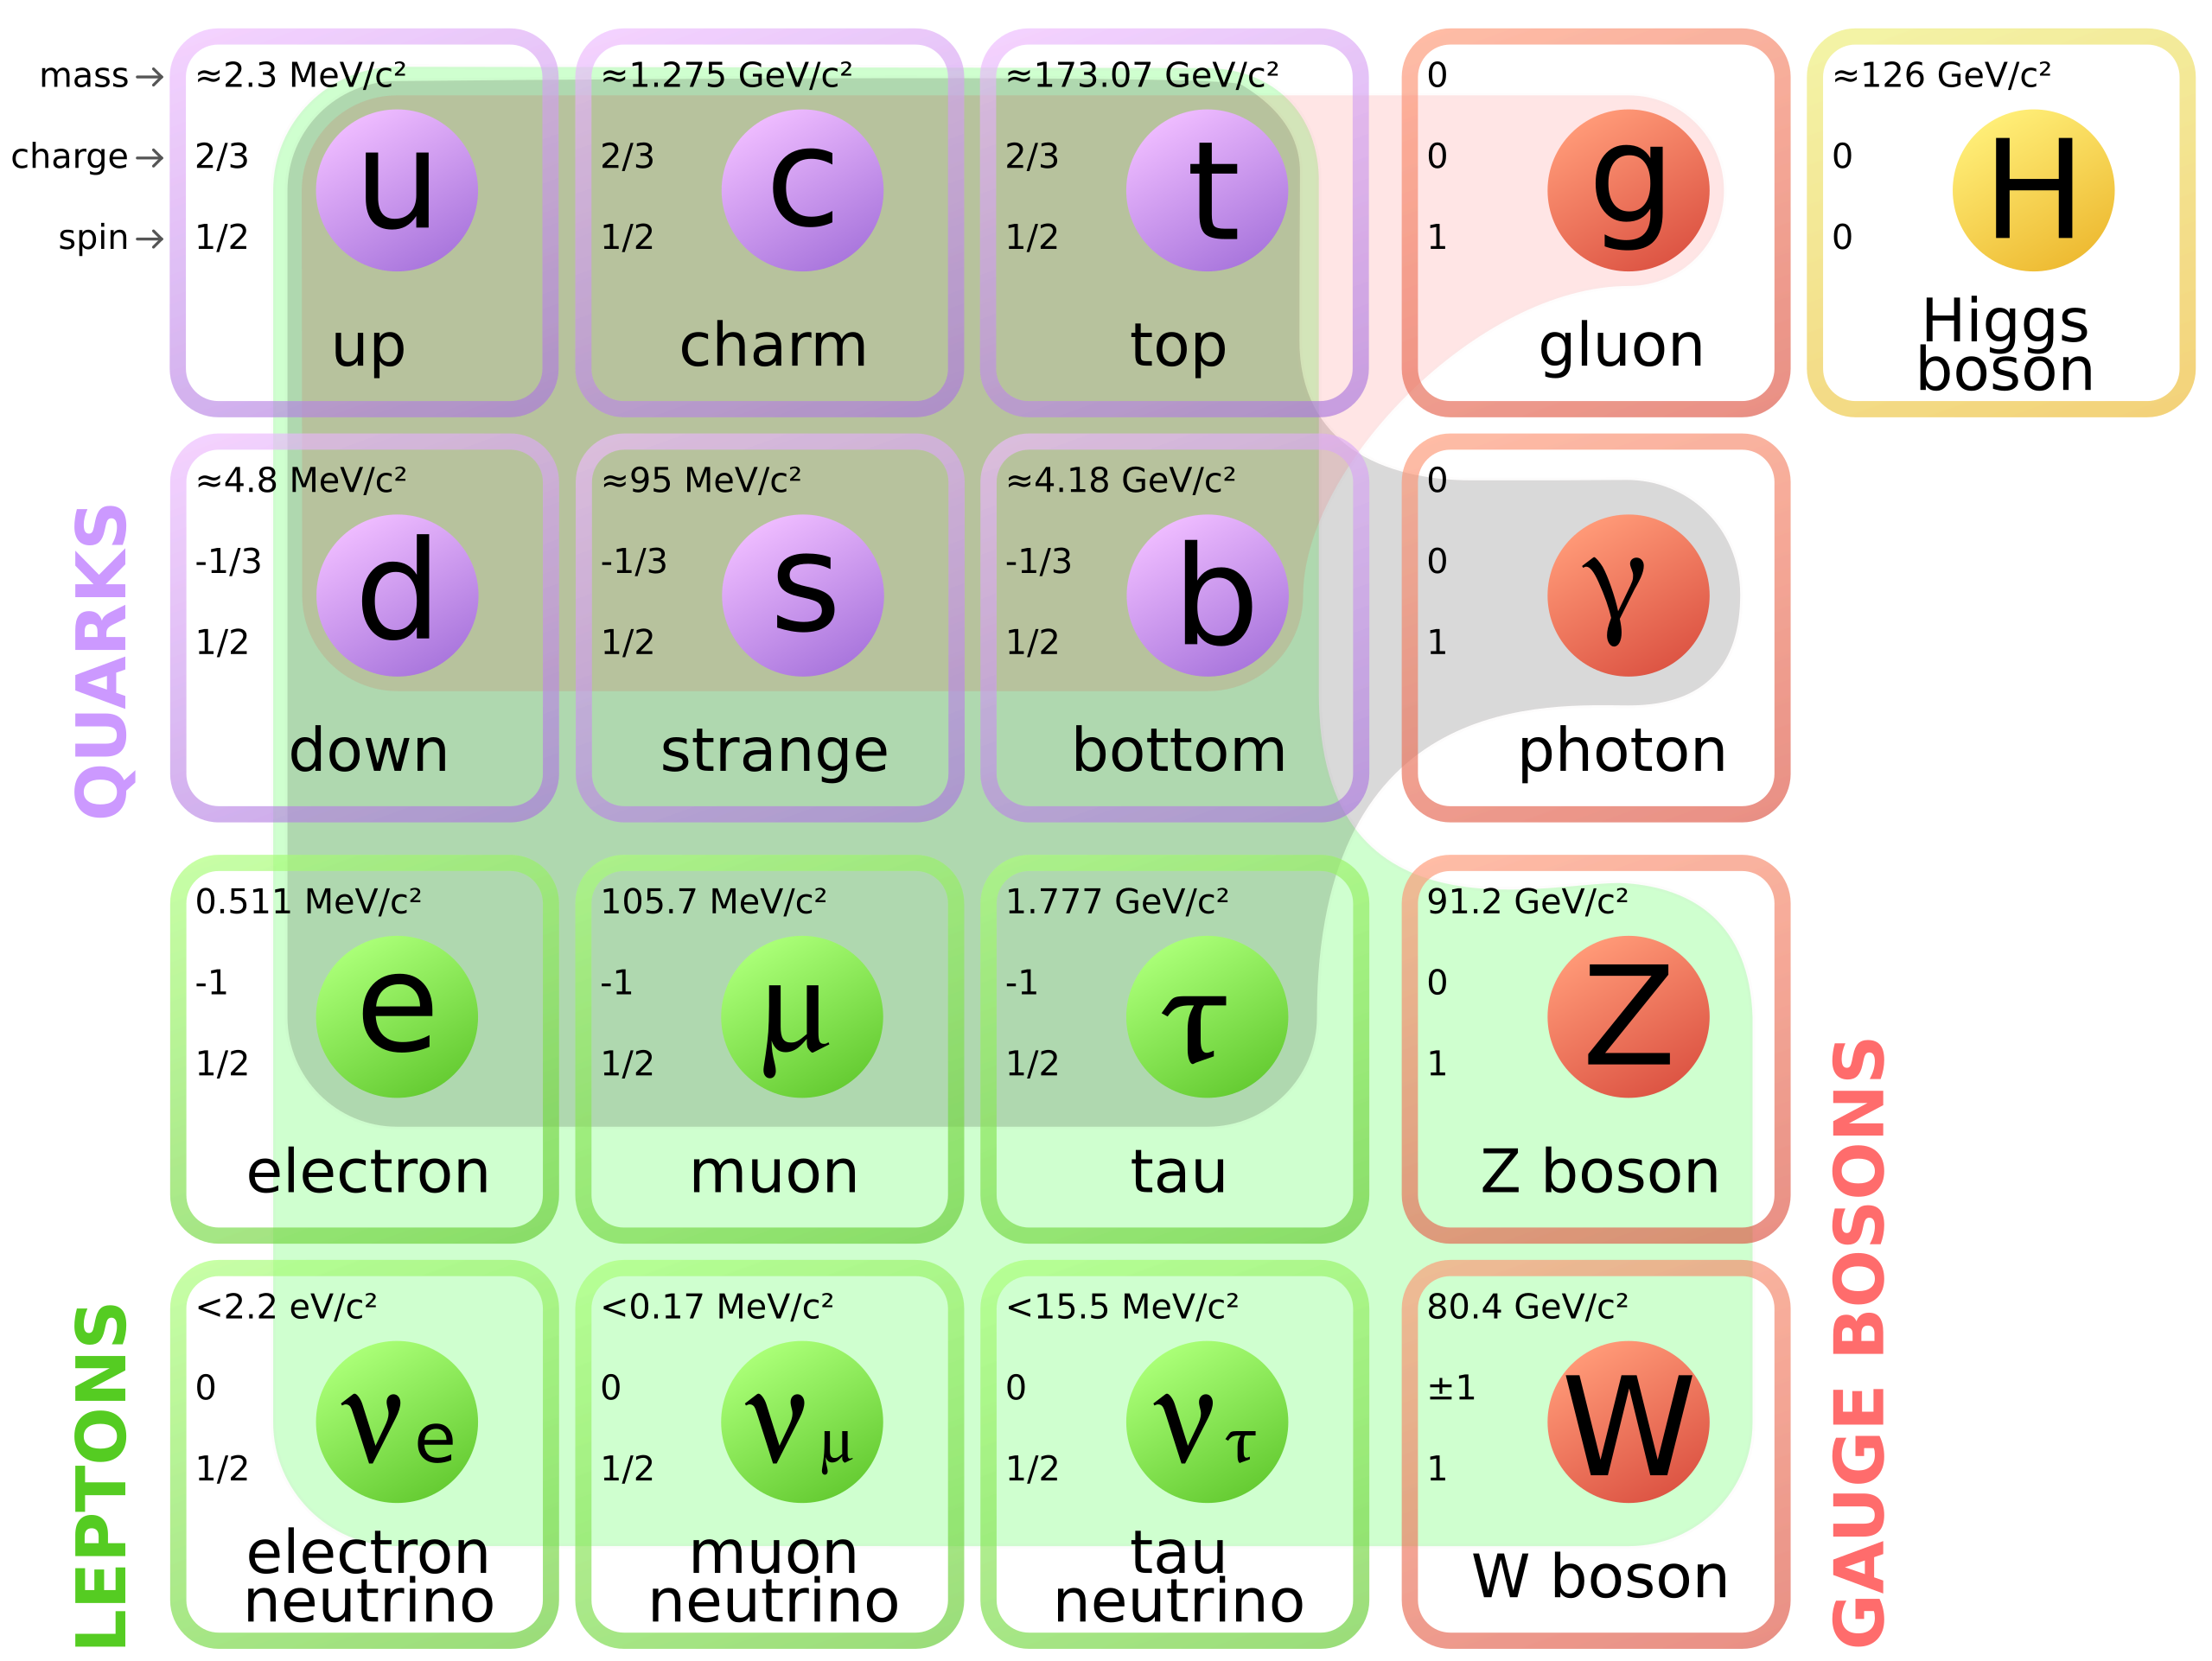
\includegraphics[width=.58\linewidth]{tabela_modeloPadrao.png}
		\caption{Fonte: \cite{WORKMAN:2022}}
	\end{figure}	
\end{frame}

\begin{frame}[plain]
	\tikzset{
		udesc greenBox/.style = {
			thin,
			blur shadow={
				shadow blur steps=10,
				shadow blur extra rounding=2pt, 
				shadow xshift=1pt
			},
			rectangle,
			minimum width=18em,
			minimum height=20mm,
			fill=greenudesc,
			text centered,
			anchor=base,
			inner sep=2ex
		},
	}
	\begin{tikzpicture}[remember picture,overlay]
		\node
			[udesc greenBox,yshift=-25pt,xshift=15pt] (box){}; 
		\node [right of = box, align=right,text=white] { {\LARGE DIS}\\Deep Inelastic Scattering};
	\end{tikzpicture}
\end{frame}
% --------------------------------------------- %
% Deep Inelastic Scattering - DIS
% --------------------------------------------- %
\begin{frame}{A Estrutura dos Hádrons}
	\framesubtitle{Deep Inelastic Scattering}
	\begin{columns}
		\column{0.4\textwidth}
		\begin{center}
			\begin{tikzpicture}[thick,scale=1, every node/.style={transform shape}]
				\begin{feynhand}
	\vertex (a1) at (0,0){$\mathrm{e^{-}}$};
	\vertex (a2) at (2,0);
	\vertex (a3) at (4,1);
	\vertex (b) at (2.5,-1.2);
	\vertex (a4) at (b);
	\uncover<2->{\vertex (a5) at (0,-1.25){$p$};}
	\uncover<3->{\vertex (a6) at (4.5,-1.25){$X$};}

	\propag [fer,  mom={$k$}] (a1) to (a2);
	\uncover<3->{\propag [fer,  mom={$k^{\prime}$}] (a2) to (a3);
	\propag [pho] (a2) to [edge label=$\gamma^{*}$] (a4);}
	\uncover<2->{\propag [fer] (a5) to (2.5,-1.25);}
	\uncover<3->{
		\propag [fer] (2.5,-1.) to (4,-1);
		\propag [fer] (2.5,-1.25) to (4,-1.25);
		\propag [fer] (2.5,-1.5) to (4,-1.5);
	}
	\uncover<2->{\vertex [blob,fill=greenudesc!40!white] at (2.5, -1.2) (c) {};}
\end{feynhand}

			\end{tikzpicture} 
		\end{center}
		\column{0.6\textwidth}
		\only<4-7>{
			\begin{align*}
				\frac{d \sigma}{d \Omega dE^{\prime}}\Bigg|_{ep\to eX}=&
				\only<4>{\left(\frac{\alpha^{2}}{4E^{2}\sin^{4}\theta/2}\right)\frac{1}{4EE^{\prime}}L^{\mu \nu}_{(L)}W^{(H)}_{\mu \nu}}
				\only<5-8>{\left(\frac{4 \alpha^{4}E^{\prime 2}}{q^{4}}\right)\left[2\sin^{2}\frac{\theta}{2}W_{1}(\nu,Q^{2})+\right. \\& \left. \quad +\cos^{2}\frac{\theta}{2}W_{2}(\nu, Q^{2})\right]}
			\end{align*}
		}
		\only<8>{
			\begin{align*}
				\frac{d \sigma}{d\Omega dE^{\prime}}&=\frac{1}{s+u}\left(\frac{4 \pi \alpha^{2}}{s^{2}t^{2}}\right)\times \\ &\quad \times \left[-(s+u)t\color{magenta}{MW_{1}(\nu, Q^{2})} \color{black}{+}\right.\\ & \left. \qquad\qquad -us\color{magenta}{\nu W_{2}(\nu,Q^{2})}\color{black}\right]
			\end{align*}	
		}
	\end{columns}
	\only<6->{
		\begin{equation*}
			\left.\begin{aligned}
					s & \equiv (p+k)^{2}=E^{2}_{cm},\\
					t &\equiv (k-k^{\prime})=-Q^{2},\\
					u &\equiv (k-p_{x})^{2}
				\end{aligned}
			\right\}
			\only<7->{\qquad s+t+u=M^{2}+W^{2}}
		\end{equation*}
	}
\end{frame}
% --------------------------------------------- %
% O DIS no Modelo de Partons 
% --------------------------------------------- %

\begin{frame}{A Estrutura dos Hádrons}
	\framesubtitle{DIS no Modelo de Partons}
	\only<1-3>{
		\begin{block}{Stanford Linear Accelerator - SLAC (1960)}
			\begin{subequations}
				\begin{align*}
					\lim_{Q^{2},\nu\to \infty}\color{magenta}{MW_{1}(\nu, Q^{2})}&\approx F_{1}(x)\\
					\lim_{Q^{2},\nu\to \infty}\color{magenta}{\nu MW_{2}(\nu, Q^{2})}&\approx F_{2}(x)\only<2-3>{\implies x\equiv \frac{Q^{2}}{2M \nu}}
				\end{align*}
				\only<3>{
					\begin{align*}
						\sigma^{\gamma^{*}p}_{L}&=\frac{4 \pi^{2} \alpha}{Q^{2}}\left[F_{2}(x,Q^{2})-2xF_{1}(x,Q^{2})\right]\\
						\sigma^{\gamma^{*}p}_{T}&=\frac{4 \pi^{2} \alpha}{Q^{2}}\left[2xF_{1}(x,Q^{2})\right]
					\end{align*}
				}
			\end{subequations}
		\end{block}
	}

	\only<4->{
		\only<4>{
			\begin{center}
				\begin{figure}[htb!]
					\centering
					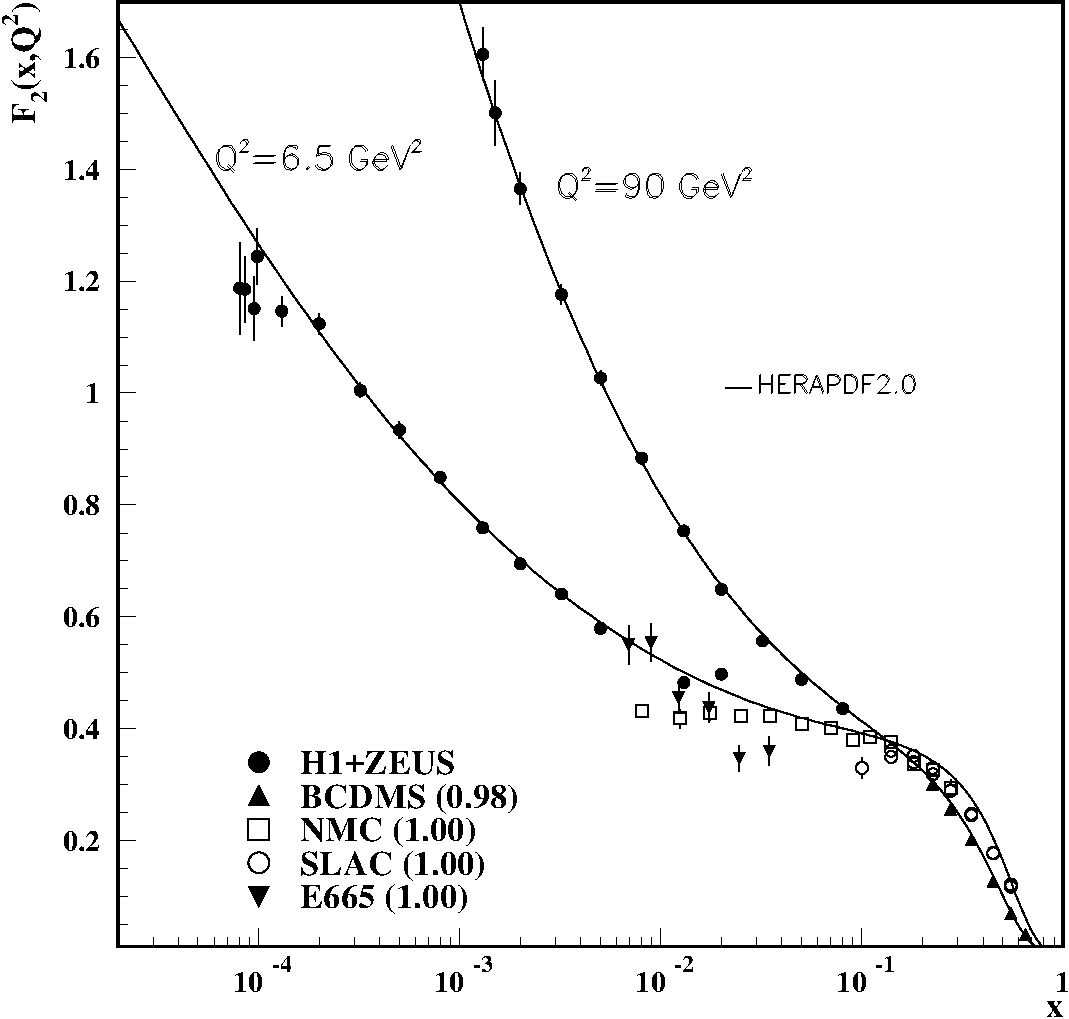
\includegraphics[width=.45\linewidth]{f2vsx.pdf}
					\caption{Fonte: \cite{WORKMAN:2022}}
				\end{figure}
			\end{center}
		}
		\only<5->{
			\begin{columns}
				\column{0.5\textwidth}
				\begin{tikzpicture}[thick,scale=1.0, every node/.style={transform shape}]
					\begin{feynhand}
	\vertex (a) {$\mathrm{e}^{-}$};
	\vertex [right=of a] (b);
	\vertex [below right=of b] (c);
	\vertex [above right=of b] (f1) {$\mathrm{e}^{-}$};
	\vertex [right=of c] (d){$\xi p+q$};
	

	\propag [fer, mom={$k$}] (a) to (b);
	\propag [fer, mom={$k^{\prime}$}] (b) to (f1);
	\propag [pho] (b) to [edge label=$\gamma^{*}(\nu)$] (c);
	\propag [fer] (c) to (d);

	\vertex (g1) at (1.35,-1.7);
	\vertex (g12) at (3.4,-1.7);

	\vertex (g2) at (1.35,-1.9);
	\vertex (g21) at (4.4,-1.9){$X(1-\xi p)$};

	\vertex (g3) at (1.35,-2.1);
	\vertex (g31) at (3.4,-2.1);

	\propag [fer] (g1) to (g12);
	\propag [fer] (g2) to (g21);
	\propag [fer] (g3) to (g31);

	% \propag [fer] (p) to (e);
	\vertex [blob,fill=red!50!white, below=1.5cm of b] (p){};
	\vertex [left=.8cm of p] (p1) {$p$};
	% \vertex [right=1.6cm of p] (e);

	\propag [fer] (p) to (c);
	\propag [fer] (p1) to (p);

\end{feynhand}

				\end{tikzpicture}
				\column{0.5\textwidth}
				\only<5->{
					\only<5-13>{
						\begin{alert}{Função Densidade Partônica (PDF):}
							\begin{align*}
								\sum_{q} \xi_{q}p&=p\\
								\uncover<6->{
								m_{q}^{2}&=(\xi p+q)^{2}=0\uncover<7->{\implies \boxed{\xi= x}}\\
							}
							\only<8>{
								\sigma^{\gamma^{*}p}&=\sum_{q}\int\limits_{0}^{1}\,d{\xi}f_{q}(\xi)\hat{\sigma}^{\gamma^{*}p}_{\color{greenudesc}{L},\color{blue!50!black}{T}}\\
							}
							\only<9-10>{
								\color{greenudesc}{\sigma_{L}^{\gamma^{*}p}(x,Q^{2})}&\color{greenudesc}{=0}\only<10>{\implies \\& \color{magenta}{F_{2}(x,Q^{2})=2xF_{1}(x,Q^{2})}}\\
								\color{blue!50!black}{\sigma^{\gamma^{*}p}_{T}(x,Q^{2})}&\color{blue!50!black}{=\frac{4 \pi^{2} \alpha}{Q^{2}}2xF_{1}(x,Q^{2})}
							}
							\only<11>{
								\sigma^{\gamma^{*}p}&=\frac{4 \pi^{2} \alpha}{Q^{2}}\color{magenta}{\sum_{q}\int\limits_{0}^{1}\,d{\xi}f_{q}(\xi)e^{2}_{q} \delta\left(1-\frac{x}{\xi}\right)}\\
								\sigma^{\gamma^{*}p}&=\frac{4 \pi^{2} \alpha}{Q^{2}}\color{magenta}{\sum_{q}e_{q}^{2}xf_{q}(x)}
							}
						\end{align*}															
					\end{alert}
				}

				\only<15>{
					\begin{figure}[htb!]
						\centering
						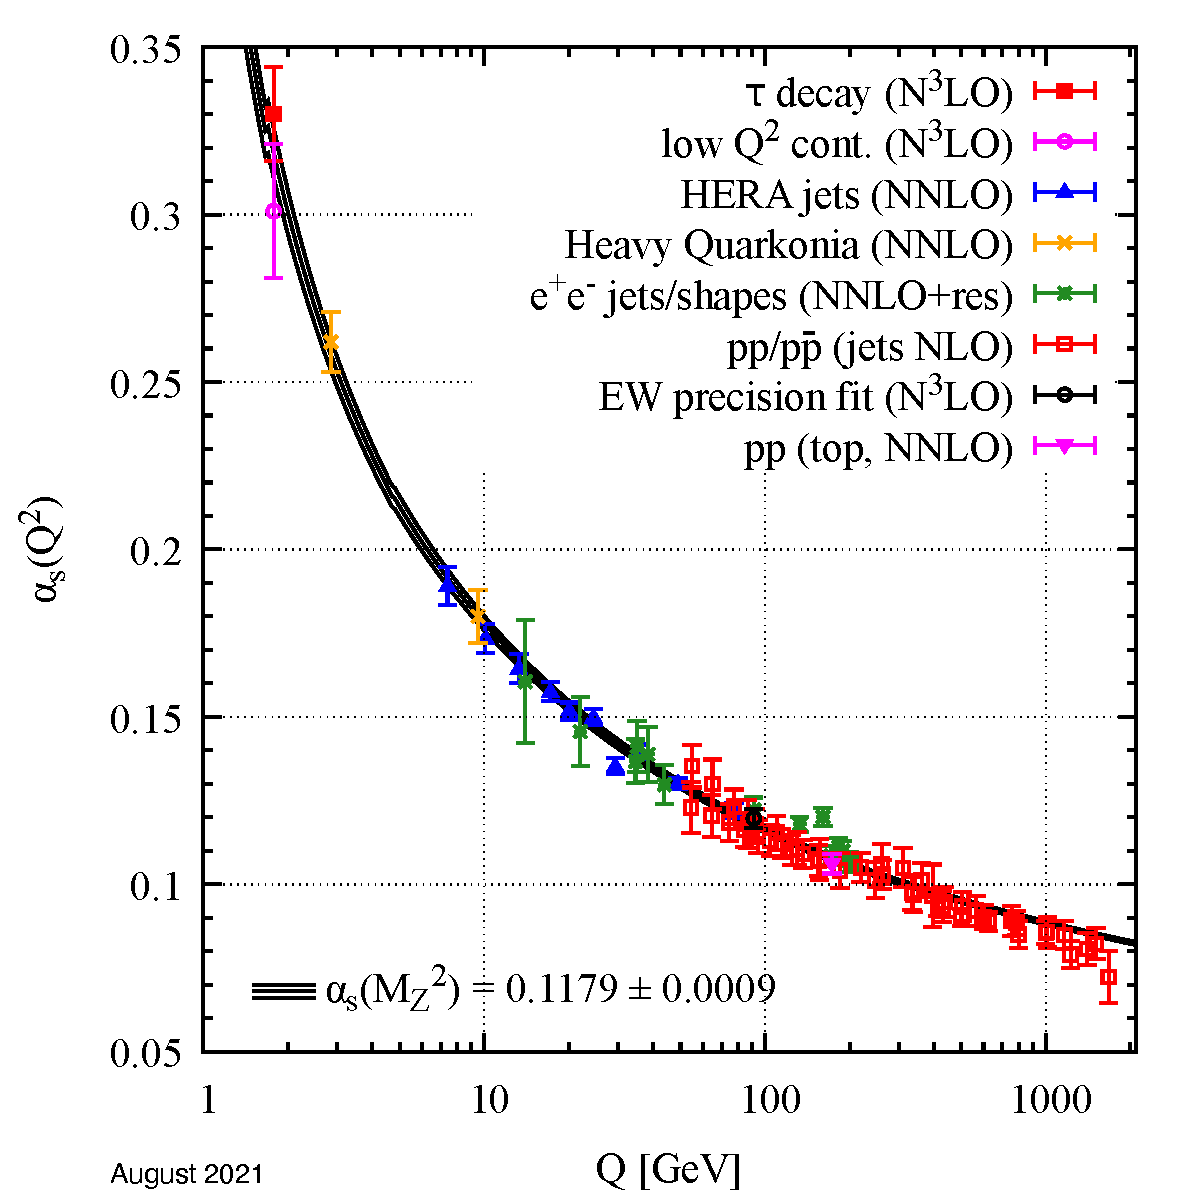
\includegraphics[width=.85\linewidth]{img/alphas-v-Q-2021.pdf}
						\caption{Fonte: \cite{WORKMAN:2022}}
					\end{figure} 
				}
			}
		\end{columns}
	}


}

% \sigma^{\gamma^{*}p}(x,Q^{2})&=\frac{4 \pi \alpha}{Q^{2}}\underbrace{F_{2}(x,Q^{2})}_{\displaystyle{2xF_{1}(x,Q^{2})}}

\end{frame}


% --------------------------------------------- %
\begin{frame}[allowframebreaks]
	\frametitle{Referencias}
	\bibliography{referencias.bib}
\end{frame}

\contato{%
	Contato: \\
	\autor{} \\
	\email{} \\
	\github{} \\
	\website{}
}

\capadetras{}

\end{document}
